\chapter{Solución del proyecto en Jetson Nano}
\label{cap:solucion-proyecto}

En este capítulo detallaremos como se ha llevado a cabo la propuesta explicada en el capítulo anterior.
Aunque existen muchas soluciones, librerías y proyectos compartidos en Python que podrían facilitar el desarrollo de este proyecto, nos hemos decantado por utilizar C\texttt{++}, debido a que estoy algo más familiarizado con esta tecnología y destaca por ser más rápida, con mejor rendimiento.
Todo eso a pesar de haber desarrollado un código bastante simple limitándonos a utilizar librerías existentes, C\texttt{++} ofrece la posibilidad de meterse más a bajo nivel para poder optimizar mejor el código, entrando más en el grano fino. Por lo que C\texttt{++} nos ha parecido una propuesta inicial interesante.

\section{Integración del Software. Dependencias}

En primer lugar, explicaremos todo el software que ha sido necesario instalar, tanto para las dependencias con el proyecto C\texttt{++} como el software necesario para hacer que el dispositivo Nvidia Jetson Nano funcionase a la perfección con el sensor Intel RealSense D435.

\subsection{Sistema Operativo. Ubuntu 18.04}

La fuente de este sistema operativo se puede obtener desde la página oficial de Nvidia, a través de \href{https://developer.nvidia.com/embedded/jetpack}{JetPack SDK} donde nos guían para llevar a cabo la instalación.
NVIDIA JetPack SDK es la solución más completa para un entorno de desarrollo completo en el desarrollo acelerado por hardware. Todos los módulos y kits para desarrolladores de Jetson Nano son compatibles con JetPack SDK.
JetPack SDK incluye Jetson Linux Driver Package con cargador de arranque, kernel de Linux, entorno de escritorio Ubuntu y un conjunto completo de bibliotecas para la aceleración de computación GPU, multimedia, gráficos y visión por computadora.

El último SDK disponible para el dispositivo Nvidia Jetson Nano es el JetPack 4.6.1, cuyo sistema operativo es Ubuntu 18.04 con versión \gls{cuda} 10.2.
El SDK JetPack 5.0 utiliza el sistema operativo de Ubuntu 20.04 con versión \gls{cuda} 11.4, pero actualmente no está disponible para Nvidia Jetson Nano, solo para modelos superiores.

\subsection{CMake. Compilador C\texttt{++}}

Como se ha mencionado anteriormente, hemos decidido elaborar el proyecto en el lenguaje C\texttt{++}. Para ello, se ha construido un proyecto utilizando CMake.

CMake es una familia de herramientas diseñada para construir, probar y empaquetar software.
Se utiliza para controlar el proceso de compilación del software usando ficheros de configuración sencillos e independientes de la plataforma.
Gracias al uso de CMake, el proyecto queda fácilmente configurado, encargándose de enlazar todas las dependencias que el proyecto necesite.
Por tanto, será necesario tener instaladas todas las herramientas necesarias para la correcta ejecución de CMake.

Además, será necesario tener instalado el compilador de C\texttt{++} para poder compilar el proyecto. El compilador instalado en el dispositivo Nvidia Jetson Nano GCC versión Ubuntu/Linaro 7.5.0-3ubuntu1~18.04.

\subsection{SDK RealSense}

Para la instalación del SDK de RealSense se ha utilizado un script que ha facilitado la instalación del mismo.
En el GitHub de \href{https://github.com/JetsonHacksNano/installLibrealsense}{installLibrealsense} podemos encontrar un script que se encarga de añadir al repositorio del gestor de paquetes las fuentes necesarias y de instalar todos los paquetes necesarios de forma automática.
Por tanto, tras clonar dicho proyecto y ejecutar el script ``./installLibrealsense.sh'' tendremos instalado por completo el SDK de RealSense.

Una vez instalado el software, podremos utilizar la aplicación RealSense Viewer para visualizar la cámara tanto en \gls{2d} como en \gls{3d}.
También podremos compilar sin problemas añadiendo las dependencias necesarias en el fichero CMakeLists.txt, como se muestra en el Código \ref{lst:dependencia-realsense}.

\begin{lstlisting}[language={C++}, caption={Dependencia CMakeLists: RealSense Library}, label={lst:dependencia-realsense}]
    # RealSense Library
    find_package(realsense2 REQUIRED)
    include_directories(include ${realsense_INCLUDE_DIR})
    target_include_directories(main PRIVATE ${realsense_INCLUDE_DIR})
    target_link_libraries(main ${realsense2_LIBRARY})
\end{lstlisting}

\subsection{Point Cloud Library (PCL)}

\gls{pcl} es una biblioteca de código abierto de algoritmos para tareas de procesamiento de nubes de puntos y procesamiento de geometría 3D, como ocurre en la visión tridimensional por computadora.
La biblioteca contiene algoritmos para filtrado, estimación de características, reconstrucción de superficies, registro 3D, ajuste de modelos, reconocimiento de objetos y segmentación.
Cada módulo se implementa como una biblioteca más pequeña que se puede compilar por separado.
PCL tiene su propio formato de datos para almacenar nubes de puntos: \gls{pcd}, pero también permite cargar y guardar conjuntos de datos en muchos otros formatos, como \gls{ply}.
También está escrito en C\texttt{++} y publicado bajo la licencia BSD.

Esta librería es muy interesante y la utilizamos tanto para aplicar filtros de pre-procesado y post-procesado, como para el método de registro \gls{icp}.

Además de tener instalada la librería, debe estar incluida como dependencia en el fichero CMakeLists.txt del proyecto de la forma que se muestra en el Código \ref{lst:dependencia-pcl}.

\begin{lstlisting}[language={C++}, caption={Dependencia CMakeLists: Point Cloud Library}, label={lst:dependencia-pcl}]
    # Point Cloud Library
    find_package(PCL 1.8 REQUIRED)
    include_directories(${PCL_INCLUDE_DIRS})
    link_directories(${PCL_LIBRARY_DIRS})
    add_definitions(${PCL_DEFINITIONS})
    target_link_libraries(main ${PCL_COMMON_LIBRARIES} ${PCL_IO_LIBRARIES} ${PCL_FILTERS_LIBRARIES})
\end{lstlisting}

\subsection{CUDA. CUDA-ICP.}

Gracias a haber instalado el sistema operativo con JetPack SDK, toda la librería de \gls{cuda} 10.2 ya viene instalada por defecto en el sistema operativo, por lo que solamente será necesario incluir como dependencia en el fichero CMakeLists.txt del proyecto de la forma que se muestra en el Código \ref{lst:dependencia-cuda}.

\begin{lstlisting}[language={C++}, caption={Dependencia CMakeLists: CUDA}, label={lst:dependencia-cuda}]
    # CUDA Library
    find_package(CUDA 10.2 REQUIRED)
    include_directories(${CUDA_INCLUDE_DIRS})
    target_link_libraries(main ${CUDA_LIBRARIES})
\end{lstlisting}

Además, encontramos un repositorio oficial de Nvidia que nos ofrece una implementación de \gls{icp} en \gls{cuda}.
Este repositorio llamado \href{https://github.com/NVIDIA-AI-IOT/cuda-pcl}{CUDA-PCL} contiene diversas implementaciones en \gls{cuda} de distintos algoritmos de la librería \gls{pcl}, entre ellos CUDA-ICP.

Nos hemos descargado de ahí la implementación \gls{icp} y la hemos importado en nuestro proyecto con las líneas en el fichero CMakeLists.txt que se muestran en el Código \ref{lst:dependencia-cuda-icp}.

\begin{lstlisting}[language={C++}, caption={Dependencia CMakeLists: CUDA-ICP}, label={lst:dependencia-cuda-icp}]
    # CUDA ICP Local Library
    target_include_directories(main PRIVATE ${CMAKE_CURRENT_SOURCE_DIR})
    add_library(libcudaicp SHARED IMPORTED)
    set_target_properties(libcudaicp PROPERTIES IMPORTED_LOCATION ${CMAKE_CURRENT_SOURCE_DIR}/lib/libcudaicp.so)
    target_link_libraries(main libcudaicp)
\end{lstlisting}

\subsection{JsonCpp}

JsonCpp es una librería que permite leer y escribir fácilmente ficheros Json en C\texttt{++}.
Esta librería no cumple ninguna función esencial para el proceso de reconstrucción de un modelo \gls{3d}, pero es muy útil ya que usamos un fichero .json donde definimos todos los parámetros que la aplicación debe tener en cuenta a la hora de ejecutarse.
Por tanto es una dependencia necesaria si se pretende compilar el proyecto tal y como se encuentra ahora mismo, ya que los parámetros se leen de un fichero .json.

Además de tener instalada la librería, debe estar incluida como dependencia en el fichero CMakeLists.txt del proyecto de la forma que se muestra en el Código \ref{lst:dependencia-jsoncpp}.

\begin{lstlisting}[language={C++}, caption={Dependencia CMakeLists: JsonCpp}, label={lst:dependencia-jsoncpp}]
    # JsonCpp Library
    find_package(PkgConfig REQUIRED)
    pkg_check_modules(JSONCPP jsoncpp)
    link_libraries(${JSONCPP_LIBRARIES})
    target_link_libraries(main ${JSONCPP_LIBRARIES})
    configure_file(parameters.json parameters.json COPYONLY)
\end{lstlisting}

\section{Desarrollo de la solución}

Tras la instalación de todo el software necesario, explicaremos detalladamente los fragmentos más relevantes del código desarrollado, siguiendo el esquema explicado en el capítulo \ref{cap:propuesta-de-solucion}, Figura \ref{fig:diagrama-propuesta-solucion}.

El programa consiste en una aplicación de consola con un pequeño menú numerado con las distintas opciones a realizar, desde la ejecución total de la reconstrucción pasando por todas las fases automáticamente tanto para la implementación de \gls{icp} de \gls{pcl} como para la implementación de CUDA-ICP, hasta la ejecución de cada una de las fases por separado, con finalidad de analizar y experimentar mejor con los resultados.

Debido a que la ejecución del algoritmo conlleva variables que no son fijas para distintos casos de uso, se ha creado un fichero json para poder personalizar los parámetros de ejecución.
A la hora de lanzar el programa, lo primero que se hace es leer el fichero json llamado ``parameters.json'' que contiene la siguiente información que se muestra en el fragmento de Código \ref{lst:parametros-aplicacion}.

\begin{lstlisting}[language={C++}, caption={Parámetros de la aplicación}, label={lst:parametros-aplicacion}]
    {
        "DataPath" : "/home/edgar/tfg/Code Solutions/JetsonNano/.data/",
        "RealSenseCaptureTotalTime_ms" : 27500,
        "RealSenseCaptureTimingBetweenCaptures_ms" : 500,
        "NumberOfCaptureFiles" : 52,
        "ResizeCenterDistance_m" : 0.63,
        "ResizeCaptureBottom_m" : 0.47,
        "ResizeCaptureTop_m" : 0.25,
        "ResizeCaptureLeft_m" : 0.5,
        "ResizeCaptureRight_m" : 0.5,
        "ResizeCaptureBehind_m" : 0.35,
        "ResizeCaptureFront_m" : 0.4,
        "ICP_Iterations" : 200,
        "ICP_MaxCorrespondenceDistance" : 0.015
    }
\end{lstlisting}

``DataPath'' especifica la ruta donde se van a guardar y tratar toda la información que sea necesaria.
Por ejemplo, si ejecutamos la fase de adquisición por separado, se guardarán ahí los ficheros para poder ser procesados posteriormente por otra fase.
El resto de parámetros los iremos viendo en este capítulo a medida que se va explicando el código.

\subsection{Adquisición de datos}

Para la fase de adquisición necesitaremos conectarnos a la cámara a través del SDK de RealSense. Para ello, inicializaremos las variables que podemos ver a continuación en el Código \ref{lst:inicializacion-adquisicion}.
``rs2::pipeline'' es la clase que se encarga de gestionar el sensor y que nos permitirá recibir los frames que está captando.
``rs2::pointcloud'' nos permitirá gestionar los frames que recibimos del sensor para convertirlos a nubes de puntos y de esta manera poder procesar el algoritmo posteriormente.
Por último, ``decimation\_filter'' se encargará de aplicar el filtro de diezmado a los frames de profundidad capturados por el sensor antes incluso de convertirlos a nubes de puntos.
Como se ha mencionado en el Capítulo \ref{cap:propuesta-de-solucion}, este es el único filtro que se ejecuta antes de la fase de pre-procesamiento, ya que se hace en el momento de la adquisición del frame.

Además de la inicialización también podemos observar un bucle inicial que se encarga de crear autoexposición en la imagen, de forma que las primeras capturas se realicen correctamente y no aparezcan oscuras o con ruido.

\begin{lstlisting}[language={C++}, caption={Inicialización del sensor RealSense D435 para la adquisición de datos}, label={lst:inicializacion-adquisicion}]
    rs2::decimation_filter decimation_filter;
    rs2::pointcloud pointcloud;
    rs2::pipeline pipe;
    pipe.start();

    std::cout << "Capturando 30 frames para autoexposicion..." << std::endl;
    for (auto i = 0; i < 30; i++) pipe.wait_for_frames();
\end{lstlisting}

A continuación, en el Código \ref{lst:bucle-adquisicion} tenemos un bucle cuya duración estará establecida por parámetro a través de la variable ``RealSenseCaptureTotalTime\_ms''.
Con la variable ``RealSenseCaptureTimingBetweenCaptures\_ms'' podemos establecer el tiempo de espera entre frame y frame que también estará establecido por parámetro.

En este bucle guardaremos los frames que recibe la cámara, aplicando el filtro de diezmado y mapeandolos a nube de puntos con RGB. Una vez obtenemos la nube de puntos, se guarda en un vector que será tratado posteriormente.

\begin{lstlisting}[language={C++}, caption={Bucle para adquisición de los datos con el sensor RealSense D435}, label={lst:bucle-adquisicion}]
    while (time < RealSenseCaptureTotalTime_ms)
    {
        std::this_thread::sleep_for(std::chrono::milliseconds(RealSenseCaptureTimingBetweenCaptures_ms));
       
        auto fs = pipe.wait_for_frames();
        auto depth = fs.get_depth_frame();
        auto color = fs.get_color_frame();

        depth.keep();
        color.keep();
        depths.push_back(depth);
        colors.push_back(color);
        pointcloud.map_to(colors[i]);
        depths[i] = decimation_filter.process(depths[i]);
        depths[i].keep();
        points.push_back(pointcloud.calculate(depths[i]));
        points[i].keep();

        i++;
    }
\end{lstlisting}

Finalmente, tenemos dos maneras de continuar con los datos. Por una parte, en el fragmento de Código \ref{lst:guardar-nubes-puntos-adquisicion} podemos ver que guarda todas las nubes de puntos almacenadas en el vector en fichero ``.ply'' para su posterior tratamiento.
Esto es útil cuando queremos separar la ejecución del programa en sus diferentes fases, ya que nos permite analizar la adquisición antes de continuar con el procesamiento de los datos.

\begin{lstlisting}[language={C++}, caption={Guardar las nubes de puntos en un fichero de datos}, label={lst:guardar-nubes-puntos-adquisicion}]
    for (i = 0; i < depths.size(); i++)
    {
        std::stringstream filename;
        filename << DataPath << "adquisitionFromRealSense/" << i << ".ply";
        points[i].export_to_ply(filename.str(), colors[i]);
    }
\end{lstlisting}

Sin embargo, cuando sabemos que el método de adquisición funciona correctamente, tenemos la alternativa de guardar las nubes de puntos directamente en memoria convirtiéndolas en nubes de puntos compatibles con la librería \gls{pcl} como podemos ver en el Código \ref{lst:tranformar-nubes-puntos-adquisicion}.

\begin{lstlisting}[language={C++}, caption={Conversión de una nube de puntos de la librería RealSense a una nube de puntos de PCL}, label={lst:tranformar-nubes-puntos-adquisicion}]
    for (i = 0; i < depths.size(); i++)
    {
        pcl::PointCloud<pcl::PointXYZRGB>::Ptr cloud_in = parseToPCLRGB(points[i], colors[i]);
        applyPreprocessingFilterTo(cloud_in);
    }
\end{lstlisting}

\subsection{Pre-procesado}

Como se ha visto a lo largo del \gls{tfg}, a pesar de estar enfocado en la reconstrucción de cuerpos humanos, también se han procesado objetos debido a su mayor facilidad ya que son cuerpos rígidos.
La adquisición de datos de estos objetos han sido tomadas desde un ángulo superior, por lo que para este tipo de datos se utiliza una matriz de rotación de 30º en el eje X para que la nube de puntos quede bien alineada inicialmente. En la subfigura \ref{fig:preprocesamiento-sin-rotar} podemos ver la nube de puntos original y en la subfigura \ref{fig:preprocesamiento-rotado} la misma nube de puntos perfectamente orientada respecto al eje X.
Para ello se usa la matriz de rotación que se muestra en el Código \ref{lst:rotacion-preprocesamiento} sobre la nube de puntos adquirida en la fase de adquisición.

\begin{figure}[h]
    \centering
    \begin{subfigure}[t]{0.33\textheight}
    	\centering
        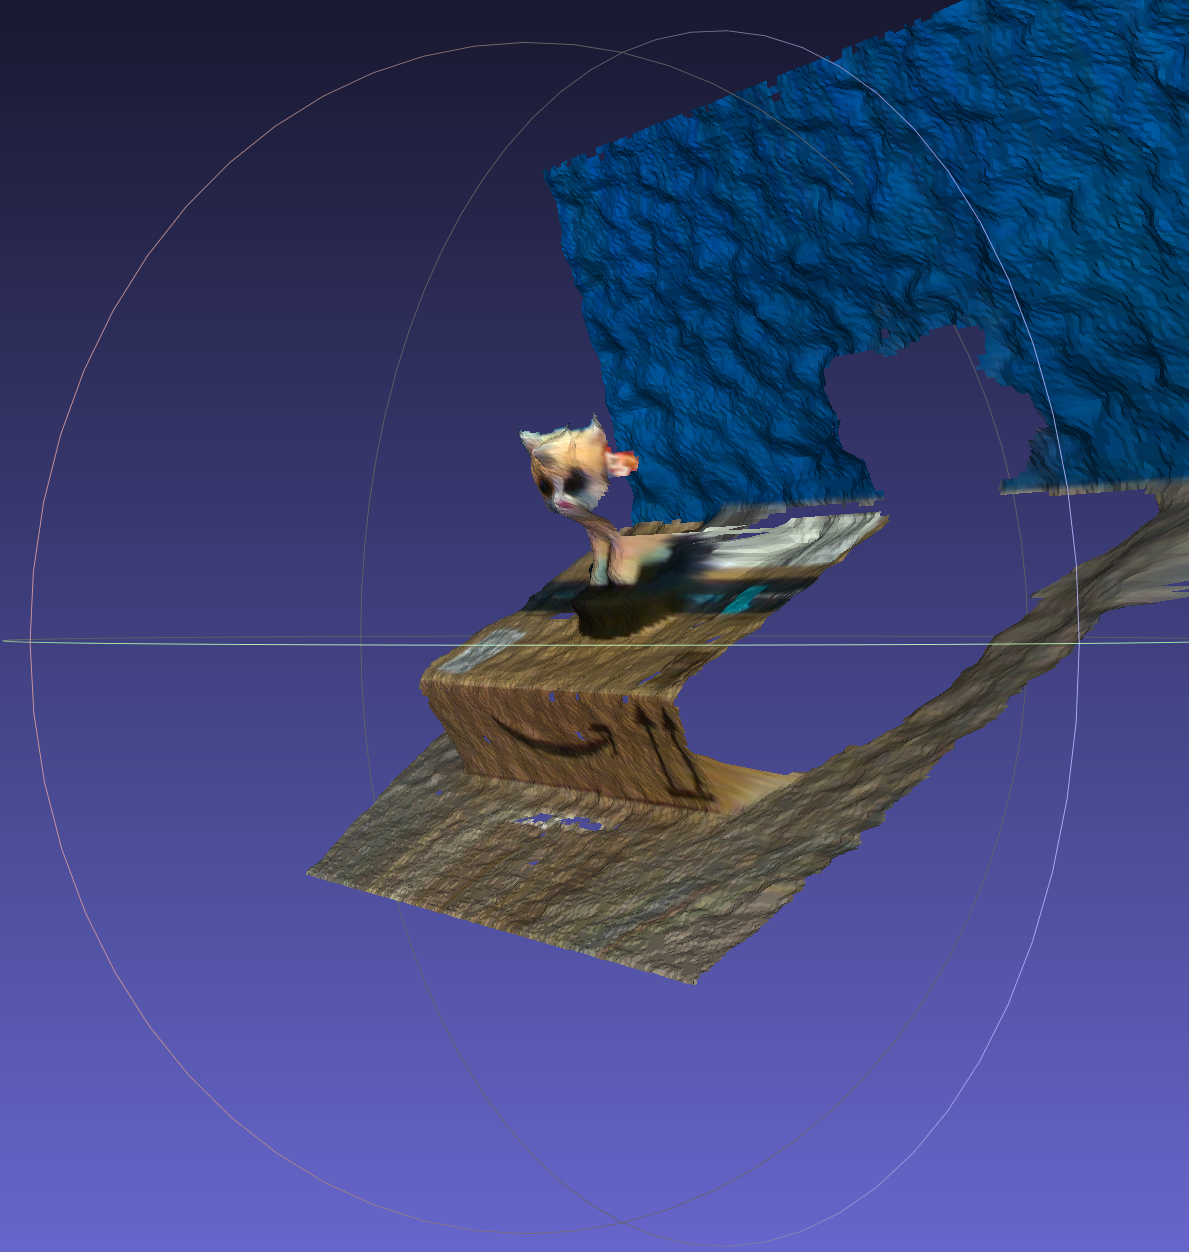
\includegraphics[height=4cm]{archivos/preprocesamiento-sin-rotar.png}
        \caption{Nube de puntos original con un ángulo de 30º desde arriba.}
        \label{fig:preprocesamiento-sin-rotar}
    \end{subfigure}
    \begin{subfigure}[t]{0.33\textheight}
    	\centering
        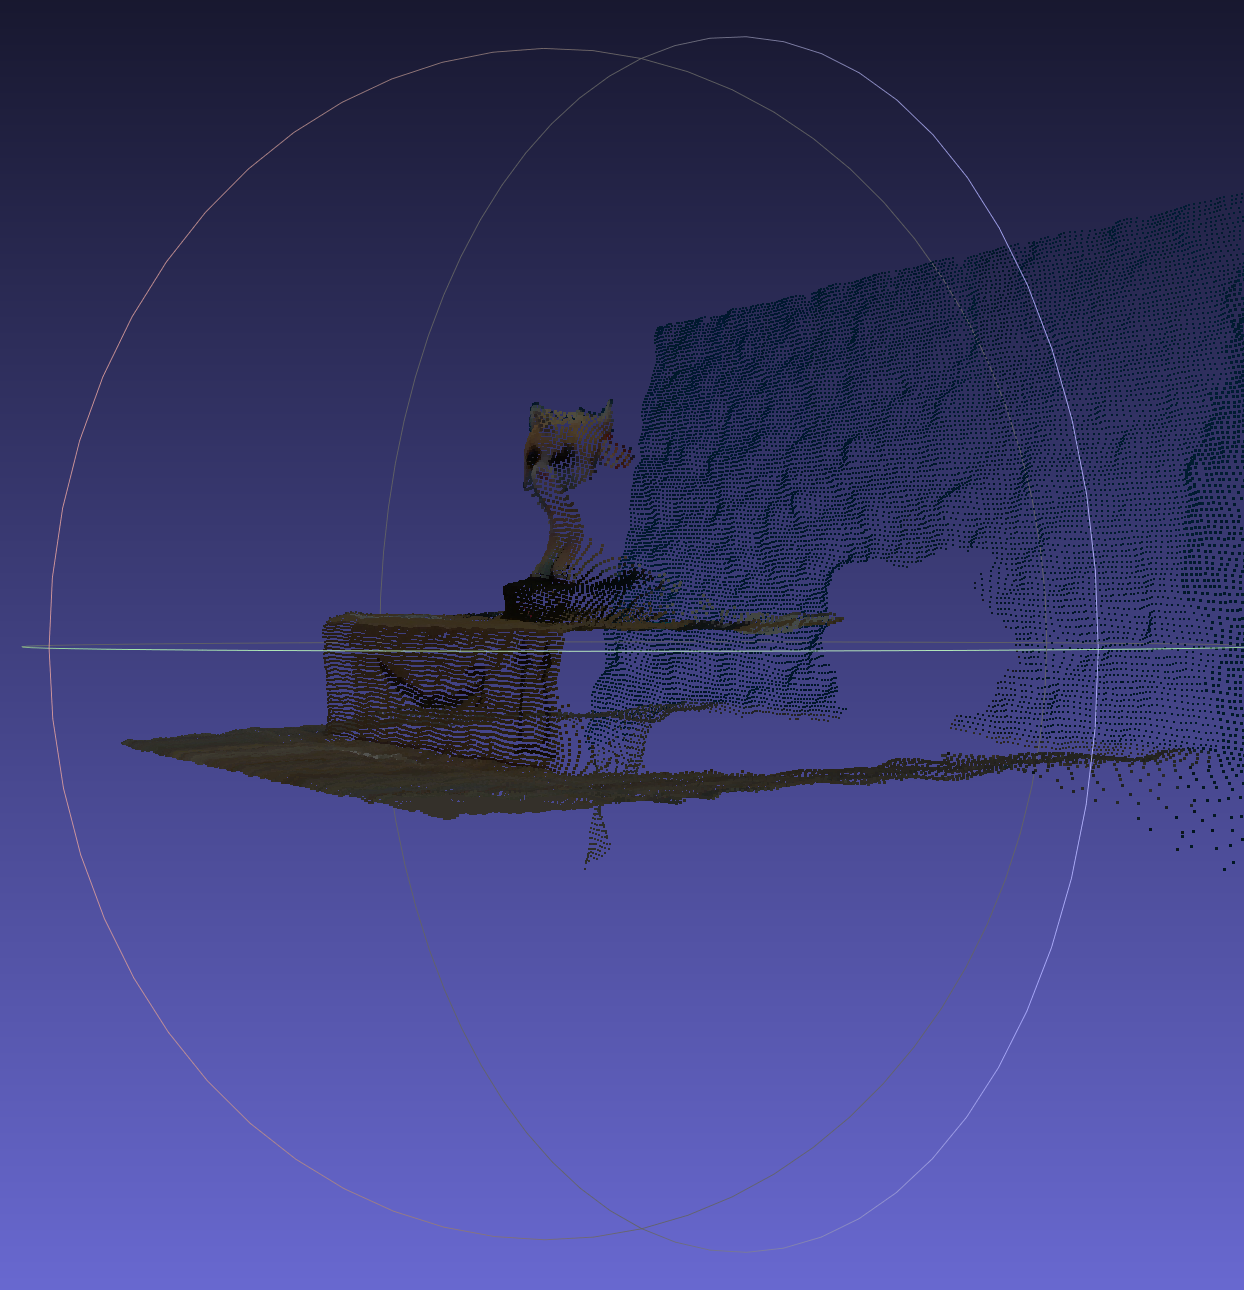
\includegraphics[height=4cm]{archivos/preprocesamiento-rotado.png}
        \caption{Nube de puntos rotada.}
        \label{fig:preprocesamiento-rotado}
\end{subfigure}
    \caption{Ejemplo de rotación en el pre-procesamiento de datos para dejar la nube de puntos alineada con el eje X.}
    \label{fig:preprocesamiento-rotar}
\end{figure}

\begin{lstlisting}[language={C++}, caption={Rotación en fase de pre-procesamiento de la nube de puntos}, label={lst:rotacion-preprocesamiento}]
    Eigen::Matrix4f transformation_matrix = Eigen::Matrix4f::Identity();
    double theta = degreesToRadians(-30);
    transformation_matrix(1, 1) = cos(theta);
    transformation_matrix(1, 2) = -sin(theta);
    transformation_matrix(2, 1) = sin(theta);
    transformation_matrix(2, 2) = cos(theta);
    pcl::transformPointCloud(*cloud, *cloud, transformation_matrix);
\end{lstlisting}

A continuación, veremos la implementación de los diferentes filtros utilizados en el pre-procesamiento de los datos. En el Código \ref{lst:passthrough} podemos ver el filtro PassThrough que nos permite limitar la nube de puntos, eliminando todos los puntos de la escena que no corresponden con el cuerpo al que queremos procesar el algoritmo \gls{icp}.
En este filtro se utilizan los parámetros del Json para establecer los límites del tamaño del cuerpo que se está procesando.

Los parámetros ``ResizeCaptureLeft\_m'' y ``ResizeCaptureRight\_m'' establecen el ancho del cuerpo a escanear en el eje X; los parámetros ``ResizeCaptureBottom\_m'' y ``ResizeCaptureTop\_m'' indican el alto del cuerpo en el eje Y; y por último los parámetros ``ResizeCaptureBehind\_m'' y ``ResizeCaptureFront\_m'' indican la profundidad del cuerpo en el eje Z. Para este último eje, hay que tener en cuenta el parámetro ``ResizeCenterDistance\_m'' que indica la distancia desde la cámara hasta el cuerpo.

\begin{lstlisting}[language={C++}, caption={Aplicación del Filtro PassThrough}, label={lst:passthrough}]
    pcl::PassThrough<pcl::PointXYZRGB> pass;
    pass.setInputCloud(cloud);
    pass.setFilterFieldName("x");
    pass.setFilterLimits(-ResizeCaptureLeft_m, ResizeCaptureRight_m);
    pass.filter(*cloud);
    pass.setInputCloud(cloud);
    pass.setFilterFieldName("y");
    pass.setFilterLimits(-ResizeCaptureBottom_m, ResizeCaptureTop_m);
    pass.filter(*cloud);
    pass.setInputCloud(cloud);
    pass.setFilterFieldName("z");
    pass.setFilterLimits(ResizeCenterDistance_m - ResizeCaptureBehind_m, ResizeCenterDistance_m + ResizeCaptureFront_m);
    pass.filter(*cloud);
\end{lstlisting}

En el Código \ref{lst:statistical-outlier-removal} podemos ver la aplicación del filtro Statistical Outlier Removal que elimina todos los puntos atípicos que se encuentran alejados del cuerpo que queremos procesar.

\begin{lstlisting}[language={C++}, caption={Aplicación del Statistical Outlier Removal}, label={lst:statistical-outlier-removal}]
    pcl::StatisticalOutlierRemoval<pcl::PointXYZRGB> sor;
    sor.setInputCloud(cloud);
    sor.setMeanK(50);
    sor.setStddevMulThresh(1);
    sor.filter(*cloud);
\end{lstlisting}

Por último, aplicamos el filtro de la Mediana que vemos en el Código \ref{lst:median-filter} para homogeneizar los puntos del cuerpo restantes en la nube de puntos.

\begin{lstlisting}[language={C++}, caption={Aplicación del Filtro Mediana}, label={lst:median-filter}]
    pcl::MedianFilter<pcl::PointXYZRGB> mf;
    mf.setInputCloud(cloud);
    mf.setWindowSize(10);
    mf.setMaxAllowedMovement(0.01);
    mf.applyFilter(*cloud);
\end{lstlisting}

Como podemos observar, todos estos filtros se utilizan desde la librería \gls{pcl}.

\subsection{Registro}

En la fase de registro comienza el procesamiento de los datos para la reconstrucción en \gls{3d} del cuerpo. En el Código \ref{lst:matriz-tansformacion-inicial} podemos ver la aplicación de la matriz de transformación inicial para todas las nubes de puntos menos la primera, ya que esta parte de 0 respecto al modelo.

\begin{lstlisting}[language={C++}, caption={Matriz de transformación inicial}, label={lst:matriz-tansformacion-inicial}]
    if (i != 1)
    {
        pcl::PointCloud<pcl::PointXYZRGB>::Ptr sourcePointCloud_transformed(new pcl::PointCloud<pcl::PointXYZRGB>);
        pcl::transformPointCloud(*sourcePointCloud, *sourcePointCloud_transformed, initialTransformationMatrix);
        sourcePointCloud = sourcePointCloud_transformed;
    }
\end{lstlisting}

Seguidamente, se procederá a efectuar el algoritmo \gls{icp} con las nubes de puntos fuente y destino, es decir, las nubes de puntos escena y modelo, respectivamente. En el Código \ref{lst:plc-icp} podemos ver la ejecución del algoritmo implementada por la librería \gls{pcl}.

\begin{lstlisting}[language={C++}, caption={Preparación y llamada al algoritmo ICP de Point Cloud Library}, label={lst:plc-icp}]
    pcl::IterativeClosestPoint<pcl::PointXYZRGB, pcl::PointXYZRGB> icp;
    icp.setMaximumIterations(ICP_Iterations);
    icp.setMaxCorrespondenceDistance(ICP_MaxCorrespondenceDistance);
    icp.setInputSource(sourcePointCloud);
    icp.setInputTarget(targetPointCloud);
    icp.align(*sourcePointCloud);
    return icp.getFinalTransformation();
\end{lstlisting}

El resultado de esta ejecución consistirá en la transformación de la nube de puntos escena (fuente), siendo alineada con el modelo (destino), y la obtención de la matriz de transformación que ha conseguido este cambio.
Una vez obtenida la matriz de transformación, nos la guardamos acumulándola con todas las anteriores para las siguientes iteraciones con las escenas restantes, como podemos ver en el Código \ref{lst:resultado-icp}.
Además, después de guardarnos la matriz de transformación sumamos los puntos de la nube de puntos modelo con la nube de puntos escena alineada, obteniendo un nuevo modelo que, poco a poco, se va completando.

\begin{lstlisting}[language={C++}, caption={Resultado del algoritmo ICP. Matriz de Transformación y nube de puntos resultante}, label={lst:resultado-icp}]
    if (i == 1)
    {
        initialTransformationMatrix = icpTransformationMatrix;
    }
    else
    {
        initialTransformationMatrix = icpTransformationMatrix * initialTransformationMatrix;
    }
    *targetPointCloud = (*targetPointCloud) + (*sourcePointCloud);
\end{lstlisting}

Por último, podemos ver la ejecución del algoritmo \gls{icp} con \gls{cuda} en el Código \ref{lst:cuda-icp}.
Lo primero que se hace es preparar los datos, pues no se envía a tratar directamente a la nube de datos de \gls{pcl}.
Se obtiene la información de los puntos en un listado de valores ``float'' y nos apuntamos la cantidad de puntos en cada nube para poder reservar la memoria suficiente para almacenar todos los puntos.
Seguidamente, reservamos memoria para la matriz de transformación y ejecutamos el algoritmo enviandole todos los datos.
Este algoritmo nos devolverá la matriz rellenada con la información sobre la transformación necesaria para alinear la escena con el modelo.
Finalmente, liberamos la memoria reservada para este proceso y se devuelve dicha matriz para continuar con el mismo procedimiento que se hace con \gls{pcl}.

\begin{lstlisting}[language={C++}, caption={Preparación y llamada al algoritmo de CUDA-ICP}, label={lst:cuda-icp}]
    int nP = pcl_cloud_source->size();
    int nQ = pcl_cloud_target->size();
    float* nPdata = (float*)pcl_cloud_source->points.data();
    float* nQdata = (float*)pcl_cloud_target->points.data();

    void* cudaMatrix = NULL;
    cudaMatrix = malloc(sizeof(float) * 4 * 4);
    memset(cudaMatrix, 0, sizeof(float) * 4 * 4);
    cudaStream_t stream = NULL;
    cudaStreamCreate(&stream);

    float* PUVM = NULL;
    cudaMallocManaged(&PUVM, sizeof(float) * 4 * nP, cudaMemAttachHost);
    cudaStreamAttachMemAsync(stream, PUVM);
    cudaMemcpyAsync(PUVM, nPdata, sizeof(float) * 4 * nP, cudaMemcpyHostToDevice, stream);
    float* QUVM = NULL;
    cudaMallocManaged(&QUVM, sizeof(float) * 4 * nQ, cudaMemAttachHost);
    cudaStreamAttachMemAsync(stream, QUVM);
    cudaMemcpyAsync(QUVM, nQdata, sizeof(float) * 4 * nQ, cudaMemcpyHostToDevice, stream);
    cudaStreamSynchronize(stream);

    cudaICP cudaIcp(nP, nQ, stream);
    cudaIcp.icp((float*)PUVM, nP, (float*)QUVM, nQ, ICP_Iterations, 1e-20, cudaMatrix, stream);

    Eigen::Matrix4f matrix_icp = Eigen::Matrix4f::Identity();
    memcpy(matrix_icp.data(), cudaMatrix, sizeof(float) * 4 * 4);
    transformation_matrix = matrix_icp;

    cudaFree(PUVM);
    cudaFree(QUVM);
    free(cudaMatrix);

    return matrix_icp;
\end{lstlisting}

En la fase de post-procesamiento se vuelven a aplicar los mismos filtros ya explicados anteriormente y finalmente se guarda la nube de puntos resultante en un fichero ``.ply'' para su análisis.
